%===================================================================================================
\subsection{Turnover}\label{model.par.turn}
%---------------------------------------------------------------------------------------------------
\subsubsection{Births \& Deaths}\label{model.par.turn.bd}
The modelled population considers ages 15--49,
reflecting commonly reported data and the majority of sexual activity.
In the absence of mortality, individuals would therefore
remain within the modelled ``open cohort'' population for 35 years.
The estimated average yearly mortality rate for these ages was 1.44\% around 2006
\cite[Table~15.2]{SDHS2006}.
However, this estimate includes HIV/AIDS-attributable mortality,
which I model separately (see \sref{model.par.hiv.mort}),
accounting for approximately 64\% of deaths around that time \cite{WHO2006esw}.
Thus, the overall exit rate from the modelled cohort
due to reaching age 50 (``aging out'') and non-HIV-attributable mortality was:
$\mu = 1/35 + (1-.64) 1.44\% = 3.78\%$.
\par
I estimated the rate of entry into the modelled population $\nu$
to fit population size of ages 15--49 in Eswatini \cite{WorldBank},
and approximate population growth rates \cite{UNWPP2019},
given that I model HIV/AIDS-attributable mortality separately.
Specifically, I assumed a population growth rate $g = \nu - \mu$ in the absence of HIV/AIDS of
4\% in 1980, 3\% in 2000, 1.5\% in 2010, and 1.5\% in 2020 (monotonic cubic interpolation).
I sampled $g$ in 2050 from a uniform prior with 95\% CI (0.7\%,~1.5\%),
reflecting uncertainty in estimated projections \cite{UNWPP2019}.
Finally, I calculated the population entry rate as $\nu = g + \mu$.
These parameter values were informally validated by comparison of model outputs with
Swati population sizes for ages 15--49 from \cite{WorldBank}.
The distribution of activity groups among individuals \emph{entering} the model, denoted $E_{si}$,
is different from the distribution among individuals \emph{currently} in the model $P_{si}$,
but $E_{si}$ is computed automatically as described below in \sref{model.par.turn.act}.
%---------------------------------------------------------------------------------------------------
\subsubsection{Activity Group Turnover}\label{model.par.turn.act}
In addition to overall population turnover (entry/exit from the open population),
I model movement of individuals between activity groups within the model.
Activity group turnover reflects the fact that risk is not constant over sexual life course,
and reported duration in higher activity contexts can be short \cite{Scorgie2012}.
Previous modelling has shown that activity group turnover (sometimes called ``episodic risk'')
can strongly influence parameter fitting and intervention impact \cite{Henry2015,Knight2020}.
I model turnover from activity group $si$ to $si'$ as a constant rate $\theta_{sii'}$,
which implies an assumption that (in the absence of HIV) duration in group $si$ is
exponentially distributed with mean $D_{si}$ \cite{Roberts2015}:
\begin{equation}\label{eq:model.par.dur}
  D_{si} = \frac{1}{\mu + \sum_{i'}\theta_{sii'}}
\end{equation}
where $\mu$ is the overall exit rate from \sref{model.par.turn.bd}.
As shown previously \cite{Knight2020}, the relative sizes of each sex-activity group $P_{si}$
can be maintained at fixed values by satisfying the following ``mass-balance'' equation:
\begin{equation}
  \nu P_{si} = \nu E_{si} + \sum_{i'} \theta_{si'i} P_{si'} - \sum_{i} \theta_{sii'} P_{si}
\end{equation}
Specific turnover rates $\theta_{sii'}$ and entrant activity group sizes $E_{si}$
can then be uniquely resolved by specifying
$N_i\,(N_i-1) = 12$ non-redundant and compatible constraints,
where specifying each $D_{si}$ is one such constraint.
%---------------------------------------------------------------------------------------------------
\paragraph{Censored Durations}
Cross sectional sex work surveys will often ask respondents about their duration in sex work.
These durations might then be taken to be the average durations in sex work;
however, this will be an underestimate,
because respondents will continue selling sex after the survey \cite{Fazito2012}.%
\footnote{An alternate example would be
  to take the mean age of a population as the life expectancy!
  Thanks to Saulius Simcikas and Dr. Jarle Tufto
  for help identifying and discussing this bias:
  \hreftt{stats.stackexchange.com/questions/298828}.}
\par
Figure~\ref{fig:diag.xdur} illustrates a steady-state population
with 5 women selling sex at any given time.
The steady-state assumption implies that a women leaving sex work after $D$ years
will be immediately replaced by a women entering sex work
whose eventual duration will also be $D$ years.
Let $D$ be this true duration, and $D_s$ be the duration reported in the survey.
If we assume that the survey reaches women at a random time point during the duration $D$,
then $D_s \sim \opname{Unif}(0,D)$,
and the mean reported duration is $\E[D_s] = \frac{1}{2}\E[D]$.
Thus, $\E[D] = 2\,\E[D_s]$ would be an estimate of the true mean duration from the sample.
In reality, sex work surveys may be more likely to reach
women who have already been selling sex for several months or years,
due to delayed self-identification as sex worker \cite{Cheuk2020}.
Thus, we would expect that $f = \E[D] / \E[D_s] \in (1,2)$,
which we can use to compute the mean exit rate as described in \sref{app.model.math.exp}.
\begin{figure}
  \centering
  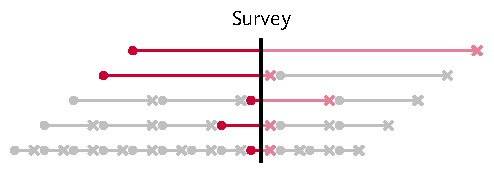
\includegraphics[scale=1]{diag.xdur}
  \caption{Illustrative steady-state population of 5 FSW,
    with varying true durations in sex work $D$,
    \vs the observed durations in sex work $D_s$ via cross-sectional survey.}
  \label{fig:diag.xdur}
\end{figure}
\par
Another observation we can make from Figure~\ref{fig:diag.xdur} is that
women who sell sex longer are more likely to be captured in the survey.
That is, while the sampled durations are representative of women who \emph{currently} sell sex,
these durations are biased high \vs the population of women who \emph{ever} sell sex.
It's not clear whether this observation is widely understood
and kept in mind when interpreting sex work survey data.
%---------------------------------------------------------------------------------------------------
\paragraph{Duration Selling Sex}
The FSW survey data for 2011 \cite{Baral2014}, 2014 \cite{EswKP2014}, and 2021 \cite{EswIBBS2022}
include questions on the respondent's current age, and age of first selling sex;
the difference between these ages can then define a ``duration selling sex''.
Using this approach, the unadjusted years selling sex among Swati FSW were
median [IQR]: 4~[2,~7] in 2011 and 5~[3,~9] in 2014,
with histograms shown in Figure~\ref{fig:fsw.yss.raw}.
However, such estimates have three sources of bias:
sampling error, censoring, and measurement error.
\par
Sampling error was addressed through RDS-adjustment in 2011 and 2021,
yielding estimates of the proportions of FSW
who have been selling sex for 0--2, 3--5, 6--10, and 10+ years.
The adjusted proportions are not significantly different between 2011 and 2021, and
indicate fewer years selling sex \vs the unadjusted proportions, which would be consistent with
challenges in reaching women in the first year(s) of sex work \cite{Cheuk2020}.
I fit an exponential distribution to the cumulative adjusted proportions
(Figure~\ref{fig:fsw.yss.adj}), yielding an estimated distribution mean
${\lambda}^{-1}$ of 4.2~(3.5,~5.3) years.
However, as discussed above, these reported years are still right censored, and
thereby underestimate the eventual duration in sex work among respondents by a factor $f \le 2$.
Thus, the overall mean duration in sex work would be given by $\bar{D} = f\,\lambda^{-1}$.
Yet, additionally, the current definition of duration selling sex
includes a hidden assumption that FSW sell sex continuously after starting.
In fact, 348/777 (45\%) FSW reported having ever stopped selling sex
in the 2014 survey \cite{EswKP2014} (other surveys did not ask).
Among these FSW, the expected duration selling sex in the current period
(\ie since re-starting most recently)
must be less than half ($\rho < 1/2$) of the durations calculated above.
Thus, an adjusted overall mean duration can be calculated as
$\bar{D} = (0.45\,\rho + 0.55)\,f\,\lambda^{-1}$.
Taking $\rho \sim \opname{Unif}(0.2,0.4)$ and $f \sim \opname{Unif}(1.5,2)$,
we obtain $\bar{D}$ with mean (95\%~CI): 5.13~(3.87,~6.72),
similar to the pooled estimate for African FSW up to 2010: 5.5~years~\cite{Fazito2012}.
\par
Finally, I assumed that higher risk FSW stay in sex work longer by a factor of
$R_{D}$ with 95\%~CI (1.54,~3.25) (gamma prior, Table~\ref{tab:fsw.ratios}).
Thus, durations in sex work among higher risk ($D_{HR}$) and lower risk ($D_{LR}$) FSW
can be resolved using:
\begin{equation}
  \begin{aligned}
    \bar{D} &= 0.2\,D_{HR} + 0.8\,D_{LR} \\
    R_{D} &= D_{HR} / D_{LR}
  \end{aligned}
\end{equation}
yielding mean (95\%~CI) $D_{LR}$: 4.07~(2.96,~5.48) and $D_{HR}$: 9.33~(6.30,~13.13) (gamma priors).
%---------------------------------------------------------------------------------------------------
\paragraph{Duration Buying Sex}
Data to inform the average duration spent buying sex among clients is limited.
\citet{Fazito2012} estimated mean durations of 4.6--5.5 years
based on studies in Benin \cite{Lowndes2000} and Kenya \cite{Voeten2002}.
\citet[Table~G]{Hodgins2022} also gives pooled estimates for
the proportions of men in Sub-Saharan Africa
who paid for sex \emph{ever} \vs in \emph{p12m} during 2000--2020.
Estimates ranged from 8.8~(6.5,~11.7)\% of men aged 25--34 who ever bought sex,
to 2.2~(1.5,~3.2)\% of men aged 35--54 who bought sex in p12m.
Based on these data, I defined a gamma prior distribution for the duration buying sex
with 95\%~CI (4,~15) years, applied to both higher and lower risk clients.
%---------------------------------------------------------------------------------------------------
\paragraph{Lowest \& Medium Activity Groups}
Data on individual-level changes to numbers of non-sex work partners in p12m
is even more sparse than data related to sex work;
so, it's unclear to what extent individuals move between the lowest and medium activity groups
throughout their sexual life course.
Data from Uganda, Zimbabwe, and South Africa \cite{Todd2009}
suggested that sexual activity (proportion sexually active and mean numbers of partners)
was approximately stable with age (after sexual debut and and before age 49),
with modest trends toward lower activity at older age.
However, these population-level data do not necessarily suggest that
the \emph{same} individuals have multiple partnerships each year.
Reflecting this uncertainty, I sampled
the rate of turnover from medium to lowest activity for both women and men
from a gamma prior with 95\%~CI (5,~50)\% per year.
%---------------------------------------------------------------------------------------------------
\paragraph{Additional Turnover Assumptions}
The above assumptions specify 3 key constraints for each sex:
two durations $D_{si}$ and one turnover rate $\theta_{sii'}$.
Since higher and lower risk FSW (and clients) are conceptualized as mutually exclusive groups,
I modelled no turnover between these groups:
$\theta_{si_{3}i'_{4}} = \theta_{si_{4}i'_{3}} = 0$ (+2~constraints).
Next, since FSW often enter sex work shortly after sexual debut \cite{Cheuk2020,Ma2020},
and sexual activity is roughly constant or slightly declining with age \cite{Todd2009},
I assumed that $E_{si} = f\,P_{si}$,%
\footnote{Subject to $f \le (\nu - \mu + D_{si}^{-1})\,\nu^{-1}$,
  which can be derived from Eq.~(10) in \cite{Knight2020}.}
with $f = 2$ for FSW, $f = 1.5$ for clients,
and $f = 1$ for medium activity women and men (+3~constraints);
then $f < 1$ for the lowest activity women and men is computed automatically.
Finally, since exiting sex work is unlikely to be
an abrupt transition to monogamous or zero sexual activity \cite{Scorgie2012,Learmonth2015},
I further assumed that (50,~90)\% of women exiting sex work
transition to the medium activity group (BAB prior) (+1~constraint);
in the absence of relevant data, I made a similar assumption regarding clients,
with (25,~90)\% former clients transitioning to the medium activity group (+1~constraint).
These $10 < 12$ total constraints then allow two degrees of freedom to resolve
the values of $\theta_{sii'}$ and $E_{si}$.
A non-negative solution to the system of constraints is solved as described in \cite{Knight2020},%
\footnote{Using \hreftt{docs.scipy.org/doc/scipy/reference/generated/scipy.optimize.nnls.html}}
repeated at each timestep as $\nu$ varies with time.
